\documentclass[a4paper,10pt]{article}
\usepackage{graphicx}
\usepackage[english]{babel}
\usepackage{subcaption}
\usepackage[latin1]{inputenc}
\usepackage[numbers]{natbib}
\usepackage{amsmath}
\bibliographystyle{unsrtnat}
\usepackage[top=1.5cm,bottom=2.5cm, left=2.5cm, right=2.5cm]{geometry}
\usepackage{siunitx}
\usepackage[parfill]{parskip}
\usepackage{multirow,float,amssymb}
\setlength{\parskip}{1em}


\begin{document}

\begin{center}
    {\textbf{\Large{A.I. notes}}}\\
    {\large{Cooper}}
\end{center}

%%%%%%%%%% Main content %%%%%%%%%%
\section{Linear Regression}
\begin{itemize}
    \item \textbf{Hypothesis} function
        \begin{gather*}
            y = h(x) = \theta_0+\theta_1x\\
            y = h(x) = \pmb{\theta}\cdot\pmb{x}\\
        \end{gather*}

        \vspace*{-0.5cm}
    \item \textbf{Loss function}
        \begin{gather*}
            J(\theta_0. \theta_1) = \frac{1}{2}\frac{1}{m}\sum_{i=1}^{m}\Big(h(x^{(i)})-y_i\Big)^2 = \frac{1}{2}\frac{1}{m}\sum_{i=1}^{m}\Big(\theta_0+\theta_1x^{(i)}-y_i\Big)^2\\
            J(\theta_0,\theta_1,\dots,\theta_N) = \frac{1}{2}\frac{1}{m}\sum_{i=1}^{m}\Big(\theta_0+\sum_{k=1}^{N}\theta_kx_k^{(i)}-y_i\Big)^2
        \end{gather*}
    \item \textbf{Calculate the Gradient} gradient is the direction along which the loss function increases the most
        \begin{gather*}
            \nabla_\theta J_{(0)} = 
            \begin{pmatrix}
                \frac{\partial J}{\partial\theta_0} \\[0.4cm]
                \frac{\partial J}{\partial\theta_1} \\
            \end{pmatrix}_{(0)}
            \hspace*{0.7cm}
            \nabla_\theta J_{(0)} = 
            \begin{pmatrix}
                \frac{\partial J}{\partial\theta_0} \\[0.2cm]
                \frac{\partial J}{\partial\theta_1} \\[0.2cm]
                \vdots \\ 
                \frac{\partial J}{\partial\theta_N} \\
            \end{pmatrix}_{(0)}
        \end{gather*}

        \vspace*{-0.4cm}
    \item \textbf{Update}
        \begin{gather*}
            \pmb{\theta}_{(1)} = \pmb{\theta}_{(0)} - \alpha\nabla_\theta J_{(0)}\\
            \pmb{\theta}_{(n+1)} = \pmb{\theta}_n - \alpha\frac{1}{m}\mathbf{X}^T(\mathbf{X}\pmb{\theta}_n-\pmb{y})
        \end{gather*}
    \item \textbf{Repeat}.
        \begin{gather*}
            \pmb{\theta}_{(n+1)} = \pmb{\theta}_{(n)} - \alpha\nabla_\theta J_{n}\hspace*{0.5cm}n = 0,1,2,\dots\\
            \text{Stop if}\hspace*{0.3cm}\left| J_{(n+1)}-J_n \right|\leq\text{tol}\hspace*{0.5cm}\text{or}\hspace*{0.3cm}n+1\geq\text{ max}
        \end{gather*}
\end{itemize}

\subsection{Regularisation}
A good machine learning model should have a good \textit{bias-variance trade-off}. This can be achieved by minimising the generalisation error, which is the sum of the squared bias and the variance. 
\begin{gather*}
    J(\theta_0. \theta_1) = \frac{1}{2}\frac{1}{m}\sum_{i=1}^{m}\Big(h(x^{(i)})-y_i\Big)^2 + \lambda\sum_{j=1}^{N}\theta_j^2
\end{gather*}
If \underline{$\lambda$ is small}, large values of $\sum_{j=1}^{N}\theta_j^2$ are allowed, meaning that the model contains too many parameters, thus it can \underline{\textbf{overfit}} (training error small, generalization error unacceptably large, high variance). If \underline{$\lambda$ is large}, only small values of $\sum_{j=1}^{N}\theta_j^2$ are allowed. This means that the training will reduce the number of parameters, this it might \underline{\textbf{underfit}} (training error is too large, high bias). 

\section{Logistic Regression}
\begin{itemize}
    \item \textbf{Hypothesis function}, models the probability that a given set of features belongs
    to class
        \begin{gather*}
            h(\mathbf{x}) = \sigma(\mathbf{\theta\cdot x}) = \frac{1}{1+exp(-\theta\cdot x)}
        \end{gather*}
    \item \textbf{Loss function} (cross-entropy), entropy measures uncertainty on the possible values of a prediction
        \begin{gather*}
            J(\theta) = -\frac{1}{m}\sum_{i=1}^{m}\Big\{y_i ln\Big[h(x^{(i)})\Big] + (1-y_i)ln\Big[1-h(x^{(i)})\Big]\Big\}
        \end{gather*}
    \item \textbf{Gradient descent} for logistic Regression:\par
    Choose a starting point $\Rightarrow$ Calculate the gradient $\Rightarrow$ Update and repeat. 
    \item If encounter \textbf{multi-class}, perform the same as many times as the number of categories of logistic regressions, each of which splits the data into two classes. End up with the same number of Hypothesis functions, select the highest probability.
    \item Metrics for classification
        \begin{itemize}
            \item Precision = $\frac{\text{True Positives}}{\text{True Positives+False positives}}$;\hspace*{0.5cm}Recall = $\frac{\text{True Positives}}{\text{True Positives+False negatives}}$
        \end{itemize}
        \begin{table}[hbt]
            \centering
            \begin{tabular}{lcccl}
            \cline{3-4}
                                & \multicolumn{1}{l|}{}           & \multicolumn{2}{c|}{\textbf{Ground Truth}}                               &  \\ \cline{3-4}
                                & \multicolumn{1}{c|}{}           & \multicolumn{1}{c|}{\textbf{1}}     & \multicolumn{1}{c|}{\textbf{0}}    &  \\ \cline{1-4}
            \multicolumn{1}{|c|}{\multirow{2}{*}{\textbf{\begin{tabular}[c]{@{}c@{}}Model\\ Prediction\end{tabular}}}} &
            \multicolumn{1}{c|}{\textbf{1}} &
            \multicolumn{1}{c|}{True Positive} &
            \multicolumn{1}{c|}{False Positive} &
            \multicolumn{1}{c}{\textbf{Precision}} \\ \cline{2-4}
            \multicolumn{1}{|c|}{} & \multicolumn{1}{c|}{\textbf{0}} & \multicolumn{1}{c|}{False Negative} & \multicolumn{1}{c|}{True Negative} &  \\ \cline{1-4}
                                & \multicolumn{1}{l}{}            & \textbf{Recall}                     & \multicolumn{1}{l}{}               & 
            \end{tabular}
        \end{table}
\end{itemize}

\subsection{Supporting Vector Machines (SVMs)}
In SVMs, we want to compute the \underline{\textbf{optimal linear decision boundary}}, which is the \textbf{hyperplane} with the largest margin between the two classes.
\begin{itemize}
    \item Support hyperplanes (optimal hyperplane between two points)
    \begin{gather*}
        \mathbf{w}\cdot\mathbf{x} + b = 1\\
        \mathbf{w}\cdot\mathbf{x} + b = -1\\
    \end{gather*}

    \vspace*{-0.8cm}
    How is the hyperplane with largest margin oriented can be found by solving an optimisation problem
    \begin{gather*}
        \text{Find }\mathbf{w},b\text{ such that }\frac{2}{\lVert w \rVert}\text{ is maximum}\\
        \text{or }\min\limits_{(w,b)}\frac{1}{2}{\lVert w \rVert}^2\hspace*{0.3cm}\text{subject to}\hspace*{0.3cm}y_i(\mathbf{w}\cdot\mathbf{x}^{(i)}+b)\geq1\hspace*{0.3cm}i = 1,2,\dots,m
    \end{gather*}
    \item Finding the hyperplane that maximizes the margin between the classes is done by minimizing a cost function, which is a convex optimization problem. Convex optimization problems have a unique global minimum, which means that the solution found by SVMs is a \textbf{global minimum}.
\end{itemize}
\begin{figure}[H]
    \centering
    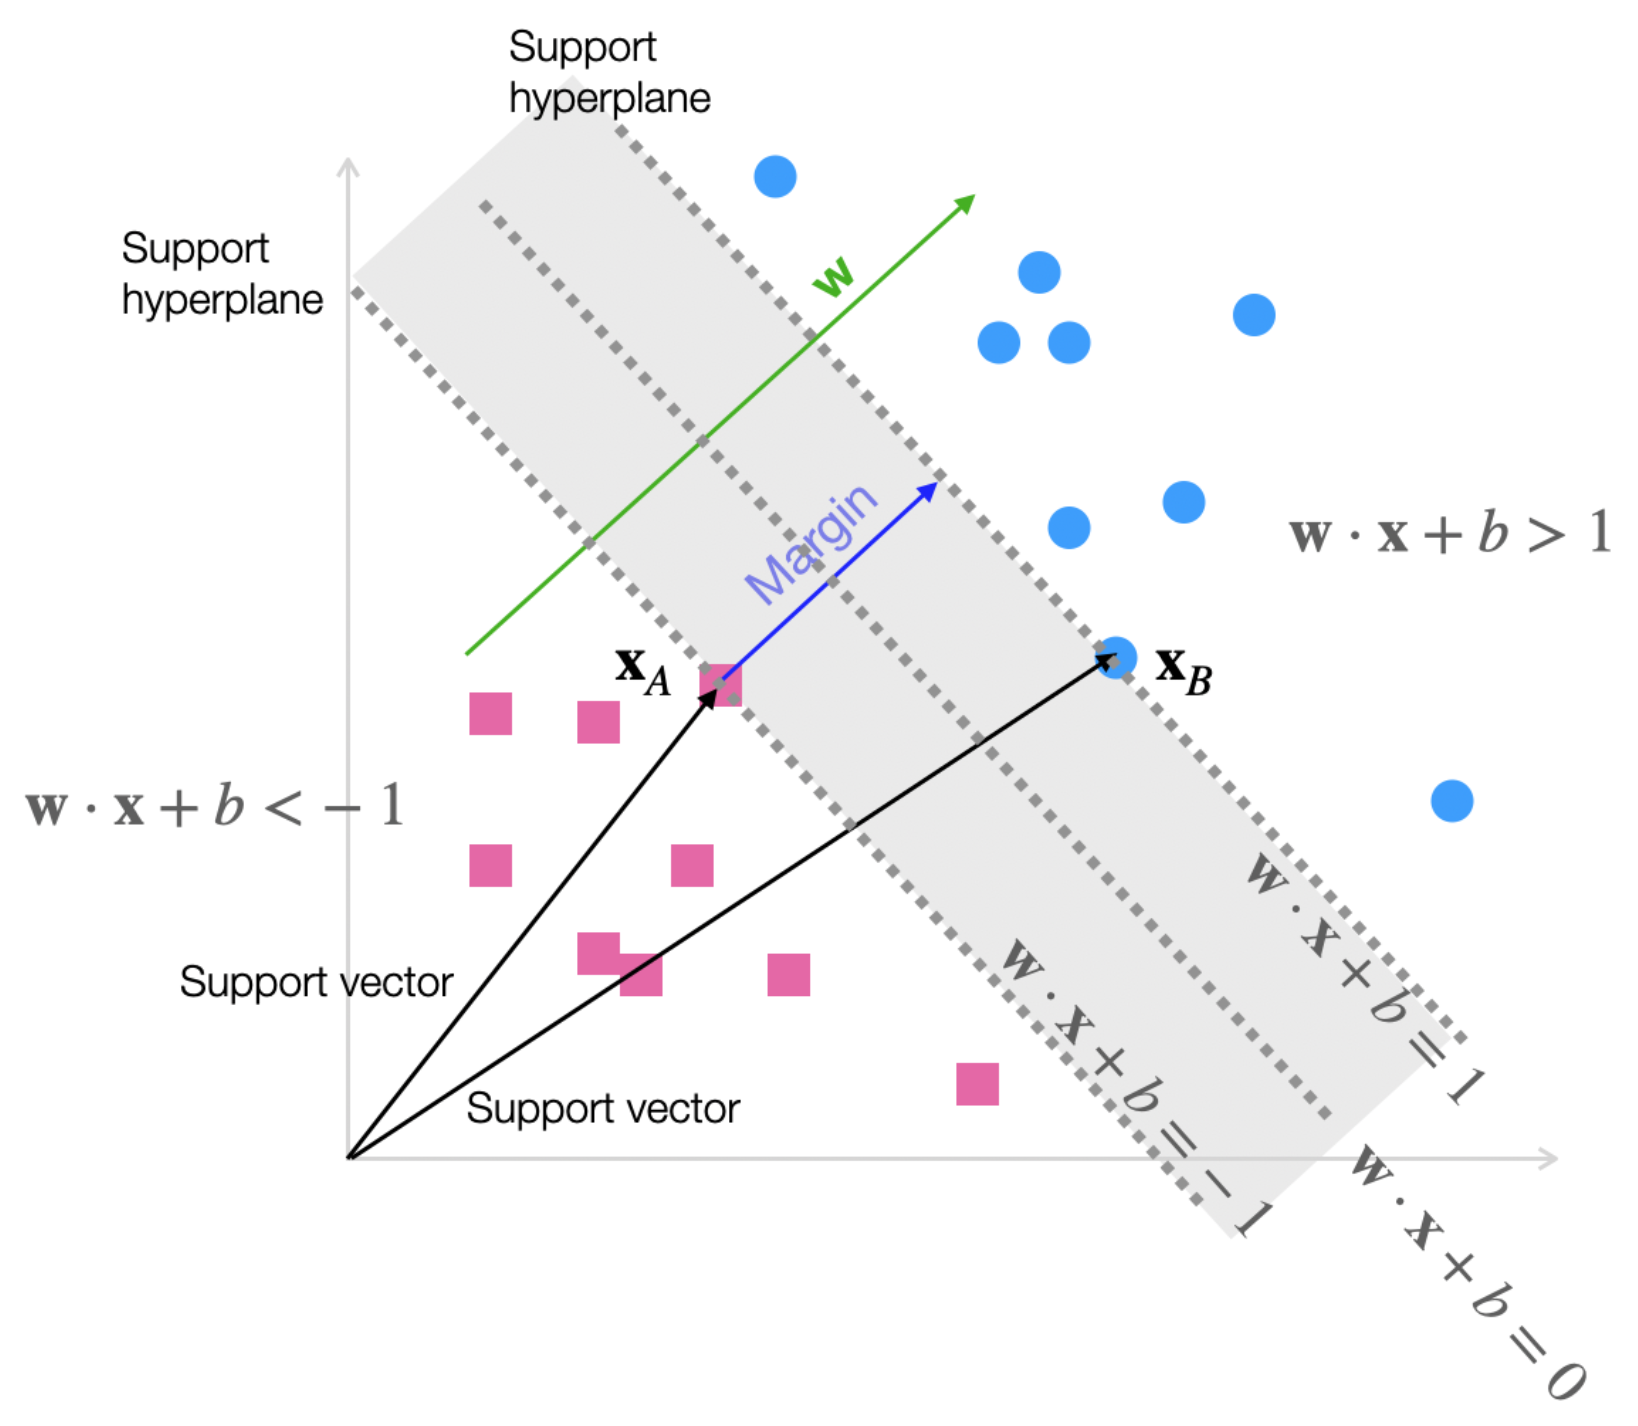
\includegraphics[width =0.55\textwidth]{svm.png}
\end{figure}

\subsubsection{Regularisation}
if the data is not linearly separable, we need to introduce regularisation to allow some misclassified data points by introducing a slack variable $\varepsilon_i>0$ such that: (i) $\varepsilon_i=0$ for correctly classified (ii) $\varepsilon_i=\left| y_i-f(\mathbf{x}^{(i)})\right|$ otherwise. 
\begin{gather*}
    \min\limits_{(w,b,\varepsilon)}\frac{1}{2}{\lVert w \rVert}^2+C\sum_{i}^{m}\varepsilon_i\hspace*{0.3cm}\text{subject to}\hspace*{0.3cm}y_i(\mathbf{w}\cdot\mathbf{x}^{(i)}+b)\geq1-\varepsilon_i\hspace*{0.3cm}\varepsilon_i\geq0\\
    \text{small C - soft (wide margin)}\hspace*{0.4cm}C\rightarrow\infty\text{ - hard margin}
\end{gather*}

\subsubsection{Kernel Trick}
For nonlinearly separable data, one option is to enrich the data with nonlinearities. This can be achieved by mapping the data into a nonlinear higher-dimensional space, $\mathbf{x}\rightarrow\mathbf{\phi(x)}$, where $\mathbf{\phi}$ is a nonlinear map, for example, a polynomial $(x_1^{(i)},x_2^{(i)})\rightarrow(x_1^{(i)},x_2^{(i)},x_1^{(i)2}+x_2^{(i)2})$. Intuitively, by adding dimensions in the feature space, it is more likely that the data becomes linearly separated.\par 

Kernel Trick decomposes the weight vector in the transformed feature space
\begin{gather*}
    \mathbf{w} = \sum_{j=1}^{m}\beta_j\pmb{\phi}(\pmb{x}^{(j)})
\end{gather*}
where $\beta_j$ become the new weights to find. In other words, we express the weight vector with coordinates defined in the transformed feature space.
\begin{gather*}
    f(\pmb{x}^{(i)}) = \sum_{j=1}^{m}\beta_j\pmb{\phi}(\pmb{x}^{(j)})\cdot\pmb{\phi}(\pmb{x}^{(i)})+b 
\end{gather*}
we resort to a theorem of functional analysis, which ensures that there exists a function, $K$, such that
\begin{gather*}
    K(\pmb{x}^{(j)}\cdot\pmb{x}^{(i)}) = \pmb{\phi}(\pmb{x}^{(j)})\cdot\pmb{\phi}(\pmb{x}^(i))
\end{gather*}
where $K$ is the \textit{kernel}. $K$ suggested that we DO NOT need to increase the dimension of the feature space to include nonlinearities, we only need to apply the kernel to inner products in the original feature space. essentially finding optimal separating hyperplane without calculating anything about $\pmb{\phi(x^{(i)})}$.\par 

\textit{Kernel} can also be explained as (i) A single-channel convolution filter, (ii) A transformation of the dataset to a higher dimension.




\section{Neural Network}
\subsection{Feedforward Neural Network}
\textit{Neural Network generalise the principle of linearly combining simple nonlinear functions}
\begin{gather*}
    y\approx h(x:\theta)
\end{gather*}
function that maps input data "x" to output "y", with the function parameters represented by "$\theta$".

\begin{figure}[ht]
    \centering
    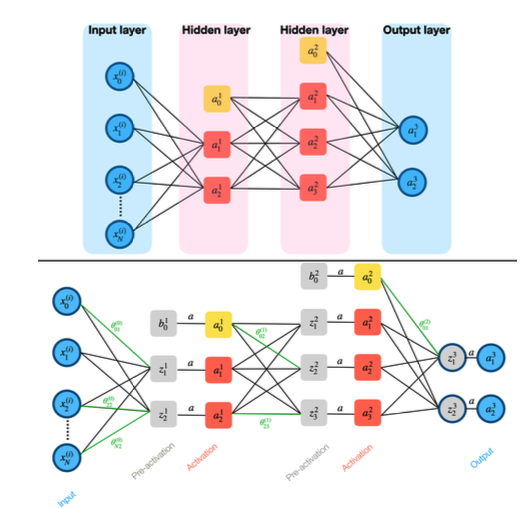
\includegraphics[width =0.8\textwidth]{FNN.png}
\end{figure}

\subsubsection{Mathematical expression}
\begin{itemize}
    \item Input layer $\rightarrow$ First hidden layer
        \begin{gather*}
            x  = 
            \begin{pmatrix}
                x_{1} \\
                x_{2} \\
                \vdots \\
                x_{m} \\
            \end{pmatrix}
            \Rightarrow\hspace*{0.4cm}\theta^{(0)} = 
            \begin{pmatrix}
                \theta_{0,1}^{(0)} & \theta_{0,2}^{(0)}  \\
                \theta_{1,1}^{(0)} & \theta_{1,2}^{(0)}  \\
                \vdots \\
                \theta_{N,1}^{(0)} & \theta_{N,2}^{(0)}  \\
              \end{pmatrix}
              ,\hspace*{0.3cm}
              z^1 = 
              \begin{pmatrix}
                b_0^1 \\
                \theta^{(0)T}x \\
              \end{pmatrix}
              ,\hspace*{0.3cm}
              a^1 = a\{z^1\} 
        \end{gather*}
    where $z$ is the \textit{pre-activation}
    \item Second hidden layer 
        \begin{gather*}
        \theta^{(1)} =
            \begin{pmatrix}
                \theta_{0,1}^{(1)} & \theta_{0,2}^{(1)} & \theta_{0,3}^{(1)}  \\
                \theta_{1,1}^{(1)} & \theta_{1,2}^{(1)} & \theta_{1,3}^{(1)} \\
                \theta_{2,1}^{(1)} & \theta_{2,2}^{(1)} & \theta_{2,3}^{(1)} \\
            \end{pmatrix}
            ,\hspace*{0.3cm}
            z^2 = 
            \begin{pmatrix}
                b_0^2 \\
                \theta^{(2)T}a^1 \\
            \end{pmatrix}
            ,\hspace*{0.3cm}
            a^2 = a\{z^2\} 
        \end{gather*}
    \item Output layer 
        \begin{gather*}
            \theta^{(1)} =
                \begin{pmatrix}
                    \theta_{0,1}^{(2)} & \theta_{0,2}^{(2)} \\
                    \theta_{1,1}^{(2)} & \theta_{1,2}^{(2)} \\
                    \theta_{2,1}^{(2)} & \theta_{2,2}^{(2)} \\
                    \theta_{3,1}^{(2)} & \theta_{3,2}^{(2)} \\
                \end{pmatrix}
                ,\hspace*{0.3cm}
                z^3 = \theta^{(2)T}a^2
                ,\hspace*{0.3cm}
                h = a^3 = a\{z^3\} 
            \end{gather*}
            Or in generalised from
            \begin{gather*}
                a^{L+1} = a\{\theta^{(L)T}a^L\}
            \end{gather*}
\end{itemize}

\subsubsection{Number of parameters}
\begin{gather*}
    \begin{split}
        \text{n. of parameters} &= \underbrace{(s_0+1)\times s_1}_{(N+1)\times 2} + \underbrace{(s_1+1)\times s_2}_{3\times 3} + \underbrace{(s_2+1)\times s_3}_{4\times 2} = (N+1)\times 2+17\\
        & = \sum_{i=0}^{L}(s_i+1)\times s_{i+1}
    \end{split}
\end{gather*}

\subsubsection{Forward propagation}
\textit{forward propagation} is the evaluation of the loss function from left to right during each iteration. 
\begin{gather*}
    J(\pmb{\theta}) = -\frac{1}{m}\sum_{i=1}^{m}\sum_{k=1}^{K}\Bigg[y_k^{(i)}\ln\Big(h_k(\pmb{x}^{(i)})+(1-y_k^{(i)})\ln\Big(1-h_k(\pmb{x}^{(i)})\Big)\Big)+\frac{\lambda}{2}\sum_{l=0}^{L}\sum_{a=0}^{s_L}\sum_{b=1}^{s_{L+1}}(\theta_{a,b}^{(l)})^2\Bigg]\\
    J(\pmb{\theta}) = \frac{1}{2m}\Bigg[\sum_{i=1}^{m}\sum_{k=1}^{K}\Big(h_k(\pmb{x}^{(i)})-y_k^{(i)}\Big)^2+\lambda\sum_{l=0}^{L}\sum_{a=0}^{s_L}\sum_{b=1}^{s_{L+1}}(\theta_{a,b}^{(l)})^2\Bigg]
\end{gather*}
Because neural networks contains nonlinear functions, the loss functions are typically \underline{\textbf{non-convex}}, a local minimum is therefore \underline{\textbf{not necessarily a global minimum}}. 

\subsubsection{Training}
Training dataset (60-80\%), Validation (10-20\%), and test (10-20\%)\par 

Initialise $\Rightarrow$ Forward propagation $\Rightarrow$ Backpropagation $\Rightarrow$ Update $\Rightarrow$ Repeat until convergence



\subsection{Convolution Neural Network}
Drawbacks from feed-forward neural networks 
\begin{itemize}
    \item textit{fully connected} layers not suitable for images: contains too many parameters  
    \item need to \textit{flatten} 2D data into 1D array --- losing spatial information. 
\end{itemize}

Generic process
\begin{itemize}
    \item input $\rightarrow$ filter (convolutional layer)$\rightarrow$ pooling layer $\rightarrow$ (repeat) $\rightarrow$ flatten $\rightarrow$ fully-connected layer
    \item Numbers of neurons in a convolutional layer
        \begin{gather*}
            N_d = \frac{W_d-F_d+2P_d}{S_d}+1
        \end{gather*}
    where $N_d$ is the number of neurons, $W$ is the width of the input channel, $F$ is the width of the filter, $P$ is the width of the pooling, and $S$ is the Stride number. 
    \item Number of parameter in convolution layer $l$
        \begin{gather*}
            l = (F_x\times F_y\times \text{n. channels} + 1 \text{ bias})\times K
        \end{gather*}
    where $K$ is the number of filters (also =number of feature maps)
\end{itemize}

\subsection{Sequence Modelling}
When both the data and its order contain information to perform the task, the points in the dataset are dependent on the position of other points in the dataset, e.g., speech recognition, DNA, time series. We lose key information if we shuffle the data.

\subsubsection{Sequence modelling with feedforward neural network}
Consider time as \textbf{feature (inputs)}, and the physical variable as \textbf{label}, may be OK for short time series, but generally not a good approach due to:
\begin{itemize}
    \item do not learn correlation as opposed to dynamical system having temporal correlations, and patterns. 
    \item large number of parameters
    \item needs the inputs of a fixed size. 
\end{itemize}

\subsection{Recurrent Neural Network}
Store the previous time-step and feed it to the next time step as the hidden state.
\vspace*{0.3cm}
\begin{gather*}
    a^{<N>} = a(\theta_a^{<N-1>}+\theta x^{<N>}+b)\\
    h^{<N>} = \theta_ha^{<N>}+b_h
\end{gather*}

\vspace*{-0.3cm}
\begin{figure}[ht]
    \centering
    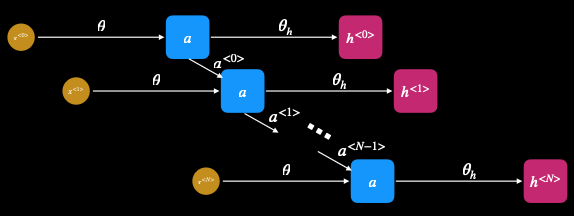
\includegraphics[width =0.6\textwidth]{RC.png}
\end{figure}

\begin{itemize}
    \item The weights and biases are shared across the time-step
    \item \textbf{time is not a feature}
    \item the loss function is a sum of the loss functions of every time step by applying chain rule across different time steps. 
        \begin{gather*}
            J = \sum_{i=0}^{N}J^{<N>}\\
            \frac{\partial J}{\partial a^{<i>}} = \frac{\partial J}{\partial a^{<N>}}\frac{\partial a^{<N>}}{\partial a^{<N-1>}}\dots\frac{\partial a^{<i+1>}}{\partial a^{<i>}} = \frac{\partial J}{\partial a^{<N>}}\underbrace{\theta_a\theta_a\dots\theta_a}_{N-i\text{ times}} = \frac{\partial J}{\partial a^{<N>}}\theta_a^{N-1}
        \end{gather*}
    \item Unstable gradient occurs from above equation, when $\theta_a$ is small, the gradient will become smaller and leads to \textbf{vanishing gradient} problem,  make it difficult for the network to remember information from previous time steps. This can be avoid by skipping some connections between layers an units, or adding a cell state to each recurrent cell. 
    \item If $\theta_a$ is large, this leads to exploding gradient, which can be solved by clip (rescale) the gradient
    \item Recurrent neural network are not ideal for learning temporal correlations in long time series due to short-term memory. 
\end{itemize}

\boxed{\textbf{NOTE:}}
\begin{itemize}
    \item 3D tensor with shape \textbf{(batch\_size, sequence\_length, input\_dim)}.
    \item \underline{\textbf{example}} refers to a sequence of input data, where each element in the sequence is a time step, e.g., audio clip, where each time step is a small segment of the audio waveform.
        \begin{itemize}
            \item In recurrent networks examples have to be input one at a time so that data in each forward propagation is still, effectively, one-dimensional
        \end{itemize}
    \item \underline{\textbf{feature}} refer to the characteristics of each time step or input element in the sequence, e.g. spectral representations of the audio waveform.
    \item \textbf{Windowing:} windowing refers to a technique of processing input data by using a sliding window over a sequence of data points. The window size determines how many data points are included in each window, and the sliding step determines how many data points the window moves forward for the next iteration. The purpose being:
        \begin{itemize}
            \item Effectively increasing the number of examples.
            \item Allowing to make predictions at any point during a sequence.
            \item Reducing the amount of data analysed at each iteration.
        \end{itemize}
\end{itemize}

\subsubsection{Long-short time memory units LSTMs}
Introducing a \textit{cell state C} to convey (store) information from the far past -- long term memory, with the combination of the same short-memory past. 
\begin{itemize}
    \item Consists of three gates to control the status of the states (forget, input, output). Each gate is controlled by a \textbf{sigmoid} activation function, due to the extreme nature of being either 1 or 0.
    \item \textbf{Forget gate.} This determines what percentage of the Long-term memory is remembered. 
    \item \textbf{Candidate state} combines the shor-term memory and the input to create a \textbf{potential long-term memory} $g$. By using \textbf{tanh} to restrain the data in the range of -1 to 1. 
    \item \textbf{Input gate} determines what percentage of the potential long-term memory is added to the long term memory $C$.
    \item \textbf{Output gate} calculates the potential long term memory from the cell state using a tanh function. Then, a sigmoid function is also used to determine what percentage of this potential long term memory is pass on as an output of the LSTM unit. 
\end{itemize}

\subsubsection{Gated recurrent units GRUs}
\begin{itemize}
    \item got rid of the cell state, and stored both long and short term memory in the \textbf{hidden state} and consists of 2 gates only.
    \item \textbf{Update gate} controls both the \textit{input} and \textit{forget} gate in determining what to forget and what to add on. 
    \item \textbf{Reset gate} decides how much past information to forget. 
    \item \textbf{Candidate state} contains past information.
    \item GRUs are simpler and with less parameters, making them easier to train than LSTMs
\end{itemize}

\vspace*{-0.3cm}
\begin{figure}[ht]
    \centering
    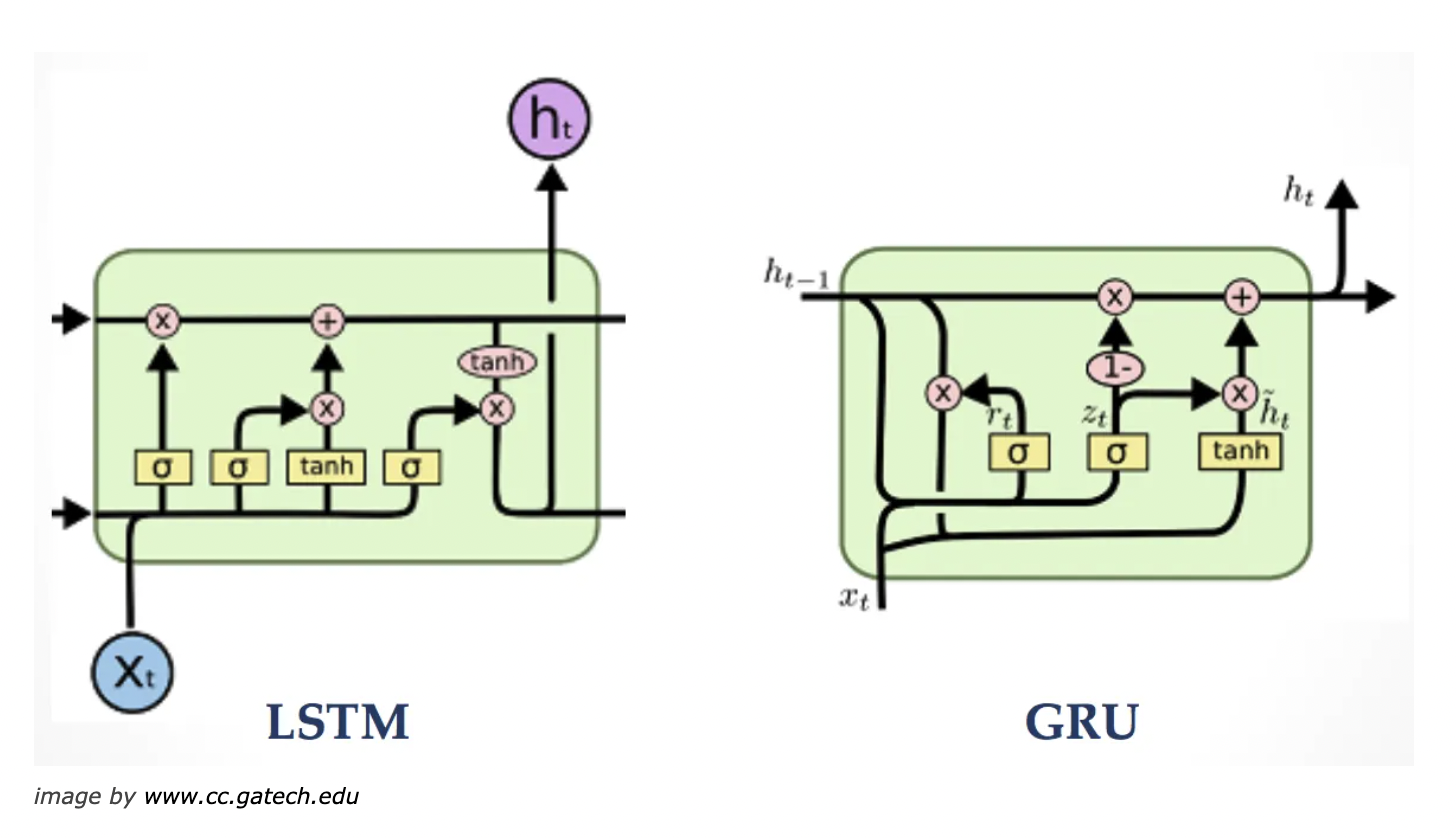
\includegraphics[width =0.7\textwidth]{LSTM_GRU.png}
\end{figure}

\boxed{\textbf{NOTE:}}\par
A GRU layer takes as \underline{input} a 3D tensor of shape \textbf{(B, T, F)}, where B is the batch size, T is the number of timestep in each sequence, and F is the number of features in each timestep. It processes each timestep in the input sequence independently and generates an output for each timestep. Therefore, the \underline{output} of the GRU layer will also be a 3D tensor of shape \textbf{(B, T, N)}, where N is the number of neurons in the layer.\par 

Types of label and its output size:
\begin{itemize}
    \item \textbf{Binary label:} For binary classification tasks, the output size of a neural network is usually 1, representing the probability of belonging to one of the two classes
    \item \textbf{Categorical label:} For multi-class classification tasks, the output size of a neural network is usually equal to the number of classes.
    \item \textbf{One-Hot encoding label:} When using one-hot encoding for multi-class classification tasks, the output size of a neural network is also equal to the number of classes, each output is binary (0 1)
\end{itemize}

\section{Unsupervised Learning}
Methods that do not require labelled dataset. \textbf{Clustering} groups the instances based on their similarity without class labels.
\subsection{k-Means clustering (Lloyd-Forgy algorithm)}
Given a set of vector-valued data, $\mathbf{x}^{(i)}$, with the goal of grouping $m$ observation into $k$ clusters. k-means algorithm is iterative and is described as following:
\begin{itemize}
    \item \textbf{Choose a metric (distance function)}. This quantitatively defines the notion of \textit{similarity} by measuring the distance between points in the \textit{feature space}. The distance are usually calculated using the squared Euclidean distance $\lVert\cdot\rVert^2$.
    \item \textbf{Choose number of clusters, $k$}
    \item \textbf{Choose the centroids} These are the baricentres (means), $\mu_j$, of the clusters, representing the positions of the clusters. 
    \item \textbf{Compute the distance} of each instance with respect to each centroid, $\lVert\pmb{x}^{(i)}-\pmb{\mu}_j\rVert^2$ for $i=1,2,\dots, k$. \textbf{Assign} each instance $\pmb{x}^{(i)}$ to the closest centroid $j$.
    \item \textbf{Compute the baricentre} of each centroid, $\mu_{j,new}=1/N_j\sum_{j=1}^{N_j}\pmb{x}^{(j)}$, where $N_j$ is the number of points, $\pmb{x}^{(j)}$, that belong in cluster j. Therefore, $\sum_{i=1}^{k}N_i=m$. 
    \item \textbf{Update centroid}. The new centroid is the baricentre from the previous new mean. 
    \item Compute the new distance, until the mean distance from the centroid stops changing. 
\end{itemize}

Although k-means algorithm presents a fast and effective method to cluster data points, it has some limits: (i) though the algorithm is guaranteed to converge, it might not be the globally optimal solution, mainly because it depends on the initial centroid initialisation and numbers of cluster chosen. (ii) it noes not perform well when clusters have varying sizes.\par 

There are several approaches to be taken to optimise the solution: (i) different centroid initialisation, (ii) number of clusters, a simple method is to plot the variance and the number of cluster, and choose the number of clusters at the inflection point (elbow). This is called the \textit{elbow method}. (iii) Feature scaling, scale the input features before running k-means. 

\subsection{Density-based spatial clustering of applications with noise (DBSCAN)}
A clustering algorithm that can handle nested clusters, and identifying nested algorithms at higher dimensions where we can't perceive by eye. DBSCAN groups points that are closely-packed, identifies the points that are isolated as outliers. 
\begin{itemize}
    \item \textbf{Choose a metric (distance function)} --- Euclidean distance, $\lVert\cdot\rVert^2$
    \item \textbf{Choose the vicinity}, $\varepsilon$ , to other points, i.e., the neighbourhood $\lVert\pmb{x}^{(i)}-\pmb{x}^{(j)}\rVert^2\leq\varepsilon$. Choose $N$ to define the number of points that are needed to classify a neighbourhood as high density. 
    \item \textbf{Select a instance} and \textbf{Count} how many instances are located with distance $\varepsilon$ from it. 
    \begin{itemize}
        \item If an instance has at least $N$ in its $\varepsilon$, then it is considered as a \textit{core instance}. All instances in $\varepsilon$ of a core instance belong to the same cluster. This may also include other core instances. 
        \item If fewer that $N$ belong in $\varepsilon$, it is identify as \textit{Non-core} instance. 
    \end{itemize}
    \item \textbf{Classify} anomalies that are not core instances. 
\end{itemize}

DBSCAN provides the advantage of not needing to specify the number of clusters, can find clusters with complicated shapes and can also identifies outliers. However, it does not cluster effectively when there are large differences in densities. 


\subsection{Hierarchical clustering}
Hierarchical clustering does not required user input cluster numbers, it does it by inspecting the result. This section will be focusing on using \textbf{Bottom-up}, in which each instance defines a cluster a iteration 0. The algorithm then paris and merge clusters. 
\begin{itemize}
    \item \textbf{Choose a metric (distance function)} --- Euclidean distance, $\lVert\cdot\rvert^2$.
    \item \textbf{Compute} the distance between all the instances. 
    \item \textbf{Merge} the closest pair into a new cluster, which is located midway its original instance. 
    \item \textbf{Repeat} Step 1-2 with $m-1$ instances. 
    \item \textbf{Stop} when left with one cluster.  
\end{itemize}

\subsection{Autoencoder}
Autoencoders are a type of neural network used for unsupervised learning, \textbf{dimensionality reduction}, and \textbf{data compression}. Composed of two main parts:
\begin{itemize}
    \item \textbf{Encoder:} takes the input data and maps it to a lower-dimensional representation. The lowest level is called the bottleneck. 
    \item \textbf{Decoder:} takes this representation and maps it back to the original input data
    \item it can perform (i)\textbf{feature reduction} and (ii) \textbf{image correction} (e.g., removal of creases in scanned documents).
\end{itemize}

\subsection{Elliptic envelope for anomaly detection}
Using Gaussian density distribution as an approach to identify outliers. 
\subsubsection{Multivariate Gaussian distribution}
A column vector of random variable (feature), $\pmb{X} = [X_1, X_2, \dots, X_N]^T$ is Gaussian distributed. 
\begin{gather*}
    f_{\pmb{x}}(\pmb{x}) = \frac{1}{\sqrt{(2\pi)^N\text{det}(\pmb{\Sigma})}}\text{exp}\Big(-\frac{\lVert\pmb{x-\mu}\rVert^2_{\pmb{\Sigma}}}{2}\Big)\sim \mathcal{N}(\pmb{\mu},\pmb{\Sigma}) ,
    \hspace*{0.7cm}
    \pmb{\mu}=\frac{1}{m}\sum_{i=1}^{m}\pmb{x}^{(i)}
\end{gather*}
where $\pmb{\mu}$ is the column-vector if the means and $\Sigma$ is the \textbf{covariance matrix}, which can be computed from a sample, $m$ (usually presented as matrix). Covariance matrix is \underline{\textbf{(1) symmetric}} and \underline{\textbf{(2) positive}}, which also represents the eigenvalues.\par
If the covariance matrix is \underline{\textbf{diagonal}} (only entries on the diagonal), then both variables are \underline{\textbf{uncorrelated}}. (different entries in the diagonal causes the circle to skew to ellipse). If the matrix is \underline{\textbf{non-diagonal}} (full) and the principal axis of the ellipse is not parallel to the frame axis, then both variables are \underline{\textbf{correlated}}
\begin{gather*}
    \pmb{\Sigma} = \frac{1}{m-1}\sum_{i=1}^{m}(\pmb{x}^{(i)}-\pmb{\mu})(\pmb{x}^{(i)}-\pmb{\mu})^T
\end{gather*}
And finally the norm that measures the distance between the mean and a feature is
\begin{gather*}
    \lVert\pmb{x}-\pmb{\mu}\rvert^2_\Sigma = (\pmb{x}-\pmb{\mu})^T\pmb{\Sigma}^{-1}(\pmb{x}-\pmb{\mu})
\end{gather*}
The inverse of the covariance matrix, $\Sigma^{-1}$, is also known as the \textit{precision} matrix. 
\subsubsection{Elliptic envelope algorithm}
elliptic envelope algorithm is a distance-based anomaly detection method that can be summarised as 
\begin{enumerate}
    \item \textbf{Assume} the datapoints to be Gaussian distributed
    \item \textbf{Compute} mean and covariance (covariance matrix also defines the shape of the ellipse)
    \item \textbf{Compute} the distance, $D$, between testpoints and the mean
    \item \textbf{Choose} the decision boundary, $c$ (the range of the elliptic)
    \item \textbf{If} $D>c$, the test point is an outlier (anomaly). 
\end{enumerate}


\section{Decision Tree}
Decision tree contains three main components: (i) \textbf{Internal nodes} that provides classification criteria, (ii) \textbf{Branches} that listed out the features that satisfies the previous criteria, and (iii) \textbf{End nodes (leaves)} that is the final result for classification. \par

Noteworthy that when classifying between binary classes, the criteria can be set for e.g., $x_1=3$ where equal sign could be used. But when dealing with numerical values, \textbf{inequalities} must be used, $x\leq3$.

\subsection{Impurity Measures}
Decision tree is constructed in the learning process node by node. The following nodes, or \textit{children nodes}, for the partition are constructed with minimum impurity. Two impurity measure will be discussed here --- \textit{information gain, Gini diversity index}
\begin{itemize}
    \item Information gain
        \begin{itemize}
            \item information gain tries to find a suitable separation line in the features that can classify data in a more effective way. e.g. by shuffling the order of the feature:
            \begin{table}[hbt]
                \centering
                \begin{tabular}{|c|c|c|c|c|c|c|c|c|}
                \hline
                $x_1$ & 3 & 7 & 3 & 4 & 3 & 6 & 5 & 6 \\ \hline
                $x_2$ & 5 & 6 & 3 & 8 & 9 & 5 & 8 & 4 \\ \hline
                label & pass & fail & pass & fail & fail & pass & fail & fail \\ \hline
                \end{tabular}
            \end{table}
            \begin{table}[hbt]
                \centering
                \begin{tabular}{|c|c|c|c|c||c|c|c|c|}
                \hline
                $x_1$ & 3 & 6 & 3 & 6 & 7 & 4 & 5 & 3 \\ \hline
                $x_2$ & 3 & 4 & 5 & 5 & 6 & 8 & 8 & 9 \\ \hline
                label & pass & fail & pass & pass & fail & fail & fail & fail \\ \hline
                \end{tabular}
            \end{table}
            In this case, we can place a separation line at $x_2\geq6$ to better separate the fail by one node. 
            \item \textbf{Entropy} can be used to evaluate the difficulty of predicting category.
            \begin{gather*}
                H(\text{label}) = -\sum_{i = 1}^{n}(p_i log_2p_i) = -\frac{3}{8}\log_2\frac{3}{8}-\frac{5}{8}\log_2\frac{5}{8} = 0.954
            \end{gather*}
            for the above example, the entropy for the separate cases are:
            \begin{gather*}
                H(\text{label},x2<6) = H_{<6} = -\frac{3}{4}\log_2\frac{3}{4}-\frac{1}{4}\log_2\frac{1}{4}=0.81,\hspace*{0.4cm}H(\text{label},x2\geq6) = H_{\geq6} = -\log_21 = 0\\[0.2cm]
                \therefore\hspace*{0.2cm}H(\text{label},x2) = 0.5H_{<6}+0.5H_{\geq6} = 0.405
            \end{gather*}
            The aim is to find features with \textbf{highest information gain} (this feature will be split into children nodes to further). \textbf{IG} is \textbf{highest} when splitting the feature makes the biggest reduction in entropy.
            \begin{gather*}
                IG(feature) = H(\text{label}) - H(\text{label}, feature) = 0.954-0.405 = 0.549
            \end{gather*}
        \end{itemize}
        \vspace*{-0.4cm}
    \item Gini Impurity Criterion
        \begin{itemize}
            \item How often a randomly chosen element from the set is incorrectly labelled. Higher GI, higher chance of misclassification
            \begin{gather*}
                GI = 1-\sum_{i=0}^{J}P_i^2
            \end{gather*}
            \vspace*{-0.4cm}
            \item Split with the lowest weighted GI for the child trees to achieve largest reduction in GI.
        \end{itemize}
    \item \underline{Shallow} trees has less variance but higher bias. \underline{Deep} trees has less bias but more prone to overfitting. 
\end{itemize}

\boxed{\textbf{NOTE:}}\par
For a classification model, high variance $\rightarrow$ overfitting, high bias $\rightarrow$ underfitting. 
\begin{itemize}
    \item If the model classifies only yellow helicopters as a helicopter.
        \begin{itemize}
            \item It is overfitting (high variance). This is because the model may be too complex and, thus, it fits features that are not relevant to the classification (the colour).
        \end{itemize}
    \item If the model classifies any round object as a helicopter.
        \begin{itemize}
            \item It is underfitting (high bias). This is because the model is unable to learn more complex feature, such as the bladed, the helicopter tail, etc.
        \end{itemize}
\end{itemize}


\section{Principal Component Analysis (PCA)}
finds an optimal direction (principle axis of the ellipsoid in gaussian distribution) of maximum variance. The maximum variance in the direction $\hat{w}_1$ is given by the maximum eigenvalue, $\lambda_1$, of the covariance matrix. Geometrically, this direction is the principal axis (eigenvector) of the ellipsoid, which is the direction along which the ellipsoid is most elongated.\par 

The difference between PCA and linear regression is:
\begin{itemize}
    \item Linear regression is sensitive on how you define input and output is large ($y=ax+b$ or $x = ay+b$), provides very different result. PCA treat variables as mathematically independent
    \item linear regression is sensitive to outliers
    \item The errors in PCA are orthogonal to the principal axis.
\end{itemize}

%%%%%%%%%% %%%%%%%%%%



\end{document}
 